\documentclass[12pt]{article}
\usepackage[utf8]{inputenc}
\usepackage{amsmath, amssymb, amsthm}
\usepackage{graphicx}
\usepackage{caption}
\usepackage{subcaption}
\usepackage{booktabs}
\usepackage[margin=1in]{geometry}
\usepackage{enumitem}
\usepackage{float}

\usepackage[colorlinks=true]{hyperref} % Improved hyperref setup

% Add this package to help with reference resolution
\usepackage{bookmark}

\title{ECS 111 Homework Assignment \#2}
\author{Kevin Oghalai}
\date{\today}

\begin{document}

\maketitle
\section{Introduction}
A logistic regression model was used to predict the probability of 
a person having an income of over \$50,000. The dataset contained age, working class, 
education, marital status, occupation, and others. It additionally contained a 
label describing the salary of the person as either over or under \$50,000.
The data was loaded in and then analyzed 
to determine possible issues that might arise from
missing values and the various types of data. 
In this case, there were multiple missing values 
in addition to many categorical variables, which could not be 
directly used for analysis. To fix this, one-hot encoding was used. 
Although data could have been filled in with the mean or median of the 
column, this would not have working for categorical variables, and in the end,
this did not end up being necessary.

\section{Data Processing}
This algorithm comes with
options to regularize the data, in addition to loss functions, optimizers, and other 
hyperparameters. In this case, the dafault values were attemped and then compared with another
and loss function. The default loss and solver were L2 loss and the lbfgs solver. 
This was compared to the liblinear solver with L1 loss, then the liblinear
solver with L2 loss. The results were then compared to the default values.

The data was split into a training and testing set. The model was trained on 
only the training set, and then the accuracy was determined on both sets later  
to investigate overfitting. As mentioned earlier one-hot encoding was used to 
deal with categorical variables. 

\section{Results}
The logistic regression model had accuracy which was fairly dependent
on the maximum number of iterations, so the results are plotted as a function 
of that. The results are shown in Figure \ref{fig:results}.


\begin{figure}[H]
\centering
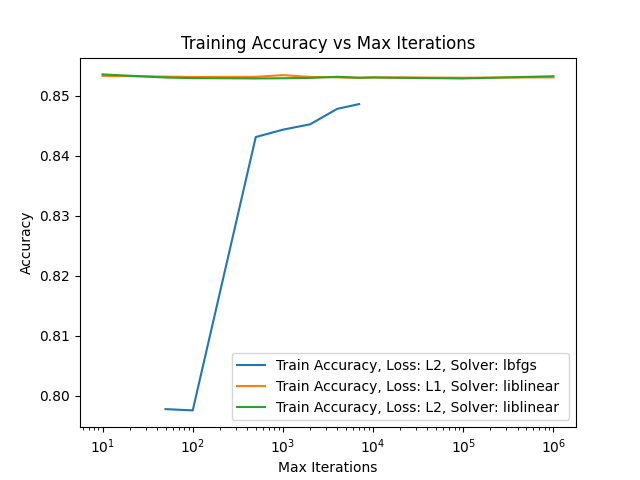
\includegraphics[width=0.8\textwidth]{train_accuracy.png} % Make sure this image exists
\caption{Training accuracy as a function of the maximum number of iterations.}
\label{fig:results}
\end{figure}

As shown in the figure above, the training accuracy ended up being higher when
using the liblinear solver, although the loss function did not seem to matter. 
Unfortunately, the L1 loss function could not be used with the lbfgs solver,
so the results are not shown. The training accuacy reached roughly 84.8\% for 
the lbfgs solver, and 85.3\% for the liblinear solver. Additionally, the lbfgs solver
ended up being too slow to run for more than 
10,000 iterations,even though it looks like it would go up more with more iterations. 
On the other hand, the liblinear solver was able to run much high numbers of iterations
in a shorter time. The testing accuracy is shown 
below in Figure \ref{fig:results2}.

\begin{figure}[H]
\centering
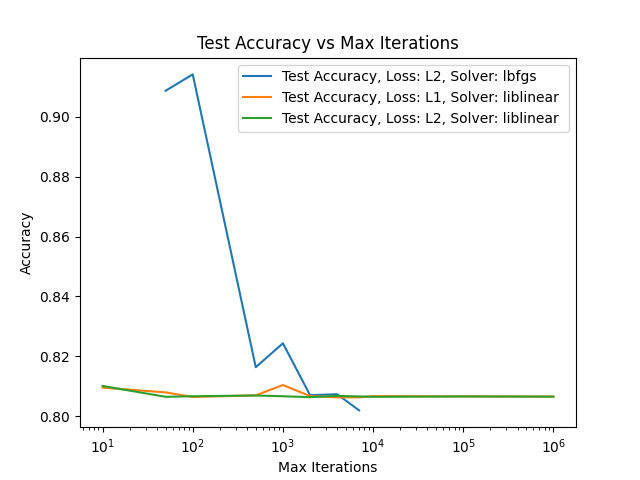
\includegraphics[width=0.8\textwidth]{test_accuracy.png} % Make sure this image exists
\caption{Training accuracy as a function of the maximum number of iterations.}
\label{fig:results2}
\end{figure}
    
Unlike above, the test accuracy actually went down with more iterations, which is 
likely due to overfitting. The test accuracy ended up going to ~81\% in all 
cases for a large number of iterations. The liblinear solver seemed to converge 
more quickly, but the lbfgs solver shows the same trend. 

\section{Discussion}

While the logistic regression model was able to achieve a high accuracy,
 it is important to note that without actually evaluating what factors the 
 model uses to determine the income, it is difficult to say why 
 exactly the income is caused. This is a classic case of correlation vs.
 causation, where the model is able to predict the income, but it is not
 necessarily able to determine the cause of the income, leading to limited 
 results being able to be drawn from the data. There is potential for misuse 
 through ignorance or malice, as this is an issue which many people are likely to care 
 about, but unable to actually analyze on their own. As an example, a reporter
 might say that getting married increases a person's salary, when in reality 
 it might be that people with higher salaries are more likely to afford to 
 get married. A slightly more humorous example would be someone buying a 
 yacht because many billionaires own yachts. The yacht would be expensive 
 and actually put the persn in debt, making them worse off.

 In order to mitigate the issue, it would be useful to analyze exactly 
 which factors cause the model to predict higher incomes. In addition, 
 experiments could be carried out tracking individuals throughout their 
 lives in order to determine which factors are causing the income and which 
 are simply correlated. This would be a difficult task, but would provide
 further insight and reduce bias.

\end{document}